%\documentclass[a4paper,12pt]{article}
\documentclass[14pt, a4paper]{extarticle}
%\documentclass[12pt,a4paper]{article}
\usepackage[utf8]{inputenc}
\usepackage[russian]{babel}
\usepackage[left=2cm,right=2cm,
    top=1cm,bottom=2cm,bindingoffset=0cm]{geometry}
    \usepackage[dvips]{graphicx}
    \usepackage{graphicx}%пакет для вставки изображений
    %\graphicspath{{piсs/}}%указываем откуда следует вставлять изображения
\DeclareGraphicsExtensions{.png,.jpg,.svg}%какое расширение будем использовать 
%\usepackage{fullpage}
\usepackage{longtable}
\usepackage{subcaption}
\usepackage[dvinames, svgnames, x11names]{xcolor}
\usepackage{pgfplots}
\usepackage{tikz}
\usepackage[unicode, pdftex]{hyperref}
\usepackage{color,soul}
\begin{document}

%\newlength{\mytextsize} % определяем высоту шрифта
%\makeatletter
%\setlength{\mytextsize}{\f@size pt}
%\makeatother
\author{Буданцев Артем}

\begin{titlepage} %Титульник

\begin{center}
{\large МИНИСТЕРСТВО НАУКИ И ВЫСШЕГО ОБРАЗОВАНИЯ РОССИЙСКОЙ ФЕДЕРАЦИИ}\\

{\small Федеральное государственное бюджетное образовательное учреждение высшего образования
«Кемеровский государственный университет»
Институт фундаментальных наук
Кафедра ЮНЕСКО по информационным вычислительным технологиям
} \\
\vspace{2cm}
{\LARGE \textbf{Отчет}}\\
по учебной практике, технологической (проектно-технологической) практике
\vspace{0.5cm}

{\large проект ``Инструменты для оформления научных статей и презентаций на примере \LaTeX'}

\vspace{4cm}

\begin{flushleft}
\textbf{Выполнили:}
\end{flushleft}
студенты направления подготовки 02.03.03 Математическое обеспечение и администрирование информационных систем 
\end{center}

\begin{flushright}
\begin{tabular}{lp{1pt}l} 
    Басалаев Дмитрий && \hspace{2cm} \\\cline{1-1}\cline{3-3} 
     {\tiny Ф.И.О.}     && {\tiny Оценка}
  \end{tabular}
  
  \begin{tabular}{lp{1pt}l} 
    Болковая Полина && \hspace{2cm} \\\cline{1-1}\cline{3-3} 
     {\tiny Ф.И.О.}     && {\tiny Оценка}
  \end{tabular}
  
   \begin{tabular}{lp{1pt}l} 
    Буданцев Артём && \hspace{2cm} \\\cline{1-1}\cline{3-3} 
      {\tiny Ф.И.О.}     && {\tiny Оценка} 
  \end{tabular}
\end{flushright}

\vspace{6cm}
\begin{center}
{\Large Кемерово 2021}
\end{center}
\end{titlepage}

\newpage%Содержание
\tableofcontents


\newpage%Првая глава
\section{``Описание проекта'}
Краткое описание: Составить презентацию и отчет о проделанной работе при помощи \LaTeX, задействовав как можно больше его возможностей.Возможно подготовить небольшую справку по интерфейсу \TeX maker.
\subsection{Актуальность, теоретическая и практическая значимость}
\textbf{Актуальность:}
Издательский пакет LateX позволяет качественно оформить любой документ или презентацию, не задумываясь о её внешнем виде, а лишь сосредоточившись на изложении и структуре. С его помощью можно легко подготовить любой документ, начиная от доклада или объемного конспекта до семестровой или курсовой работы с многочисленными формулами.
\subsection{Теоретическая значимость}
\begin{itemize}
  \item Знакомство студентов с издательским пакетом \LaTeX, описание его преимуществ и недостатков
 \item Получение нами умения создавать качественные pdf документы
\end{itemize} 
\subsection{Состав группы участников проекта}
\subsection*{Состав группы}
\begin{tabular}{| l| l| l| l|}
\hline {\bfseries \large №} & {\bfseries \large ФИО} & {\bfseries \large \textsl{группа}} & {\bfseries \large Логин на github.com } \\ \hline
1. & Басалаев Д.А.  & МОА-205 & FySyZe \\ \hline
2. & Болковая П.А.  & МОА-205 & ApollinariaB \\ \hline
3. & Буданцев А.А.  & МОА-205 & Antur1um \\ \hline
\end{tabular}
\subsection{Общие цель и задачи}
\textbf{Цель:} Составить презентацию и отчет о проделанной работе при помощи LateX, задействовав как можно больше его возможностей.
\subsection{Распределение по ролям}
\textbf{Басалаев Д.А.} Работа с презентациями, форматирование страницы\\
\textbf{Болковая П.А.} Работа с изображениями и встроенной графикой\\
\textbf{Буданцев А.А.} Ввод формул, построение графиков, различные окружения
\subsection{План-график работы}
\begin{tabular}{| l| p{13cm}|}
\hline {\bfseries \large Даты} & {\bfseries \large Действия}\\ \hline
03.02.21-11.03.21. & Изучение базы, установка необходимого софта,подготовка документации\\ \hline
12.03.21-26.03.21 & Изучение интерфейса в \TeX maker, набор простых текстов, спецсимволы \\ \hline
27.03.21-15.04.21 & Ввод математических формул, ввод матриц, спецсимволы  \\ \hline
16.04.21-28.04.21 & Работа с изображениями и встроенной графикой, построение графиков \\ \hline 
29.04.21-14.05.21 & Работа с ссылками, разметка страницы, различные окружения, работа с презентациями \\ \hline
15.05.21- & Разработка финального продукта, подготовка отчета. \\ \hline
\end{tabular}
\subsection{Что такое \TeX и \LaTeX ?}
\textbf{\TeX} — издательская система, созданная американским математиком и программистом Дональдом Кнутом (Donald E. Knuth). TEX был разработан, преследуя две основные цели: - позволить всем создавать качественные публикации с разумными для этого усилиями. \TeX знаменит своей чрезвычайной стабильностью, работой на различных операционных системах и практически полным отсутствием ошибок. Одна из главных причин по которой \TeX выбирают для оформления научных работ заключается в том, что с его помощью можно достаточно легко вводить сложные формулы.\\

\textbf{\LaTeX} — наиболее популярный набор макрорасширений (или макропакет) системы компьютерной вёрстки \TeX, который облегчает набор сложных документов.Первая версия \LaTeX была написана в 1984 году Лесли Лампортом (Leslie Lamport) и с тех пор стала доминирующим способом подготовки \TeX публикаций. Важно заметить, что ни один из макропакетов для \TeX ’а не может расширить \TeX ’овских возможностей (всё, что можно сделать в LaTeX’е, можно сделать и в \TeX ’е), но, благодаря различным упрощениям, использование макропакетов зачастую позволяет избежать весьма изощрённого программирования.Пакет позволяет автоматизировать многие задачи набора текста и подготовки статей, включая набор текста на нескольких языках, нумерацию разделов и формул, перекрёстные ссылки, размещение иллюстраций и таблиц на странице, ведение библиографии и др. Кроме базового набора существует множество пакетов расширения \LaTeX.

\subsection{Используемые программные средства}
\begin{itemize}
\item[1.]Github

\item[2.]\TeX Live

\item[3.]\TeX maker
\end{itemize}
Для того чтобы использовать \LaTeX на современном ПК под управлением Windows 10 нам понадобится загрузить и установить \TeX live maneger(это наиболее полный дистрибутив \LaTeX), а также \TeX maker(это редактор для создания TEX документов). А для сохранения документов в формате pdf нам понадобится написать пару строк в командной строке.

\subsection{Что представляет собой \LaTeX докумет}
\LaTeX документ состоит из двух частей: файл с расширением .tex в котором содержатся обычный текст и команды \LaTeX(входной файл) и собственно скомпилированный pdf файл(выходной файл). Для того чтобы получить pdf файл из .tex файла нам необходимо зайти в командную строку, затем при помощи команды "cd" перейти в директорию в которой лежит .tex файл затем написать команду "pdflatex" и название файла с указанием расширения (.tex).(например: pdflatex FinalReport.tex)

\section{Ход работы}

\subsection{03.02.21-11.03.21}
Загрузили \TeX live maneger и \TeX maker. Ознакомились с интерфейсом, синтаксисом набора команд и структурой документа. Подготовили документацию по проекту.

\subsection{12.03.21-26.03.21}
Изучили набор команд для написания спец. символов и изменения шрифта(\{ \textbf{жирный}, \textsl{Курсив}, {\tiny крошечный} {\Huge Огромный} \} \$ \texteuro \   и др.)
Решили составить таблицу, содержащую наиболее часто используемые команды, но вскоре отказались от этой идеи ибо в \TeX maker присутствуют автоматические подсказки, а также многие действия вынеcены на кнопки интерфейса. 




\begin{figure}[h]
\begin{tabular}{cc}
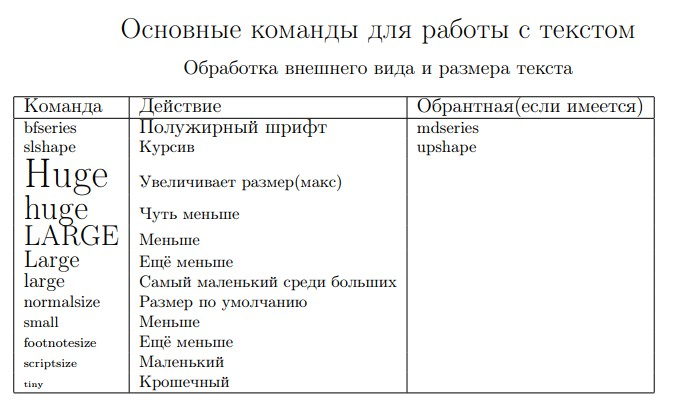
\includegraphics[width=9cm,height=7cm]{table(1)}
&
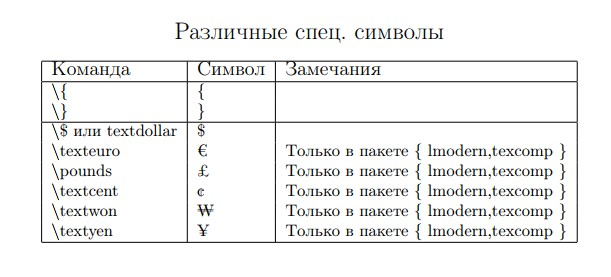
\includegraphics[width=9cm,height=7cm]{table(2)}
\end{tabular}
\caption{Та самая недоделанная таблица}
\end{figure}
\newpage
\begin{figure}[h!]
\setlength{\fboxsep}{0pt}%
\setlength{\fboxrule}{1pt}%ширина рамки
\fbox{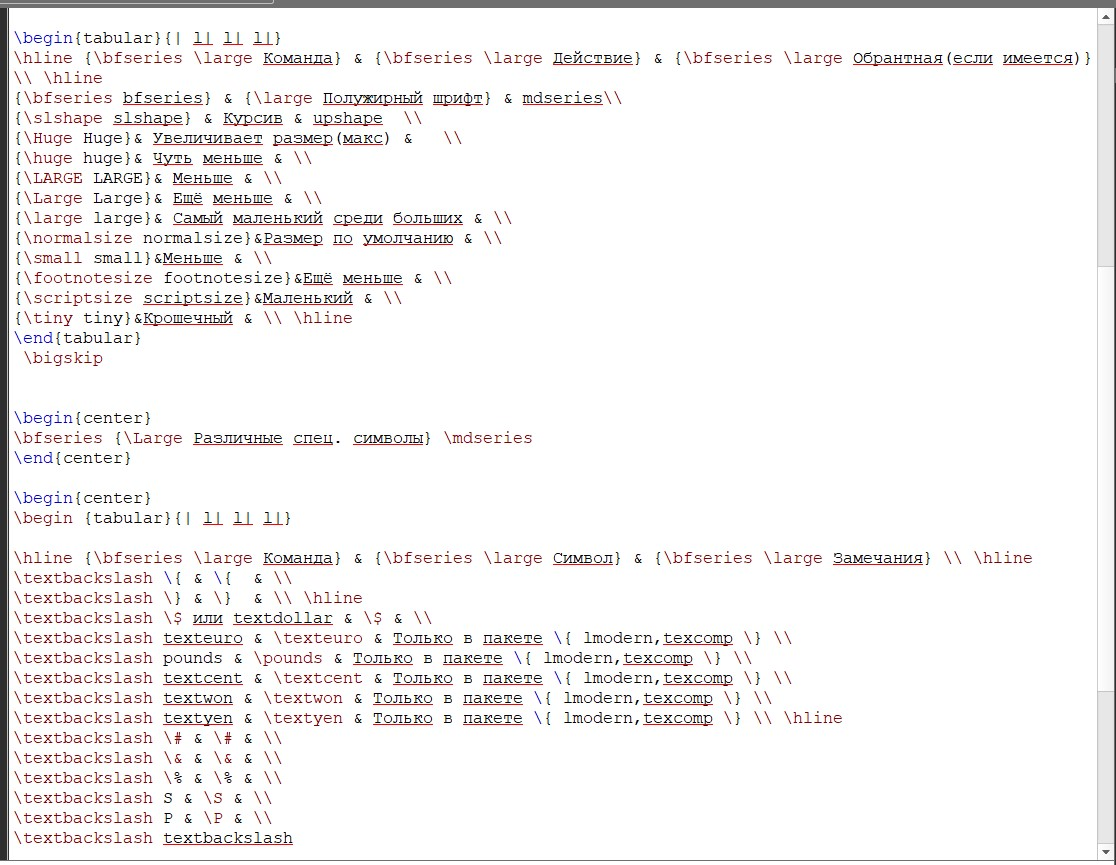
\includegraphics[width=15cm,height=9cm]{TableCode}}%
\caption{Код таблицы}
\label{fig:image}
\end{figure}




\subsection{27.03.21-15.04.21}
Итак, мы приступили к вводу математических выражений и формул. Желая начать с чего-то простого мы решили переписать школьную таблицу производных и интегралов.
\begin{figure}[h!]
\setlength{\fboxsep}{0pt}%
\setlength{\fboxrule}{1pt}%ширина рамки
\fbox{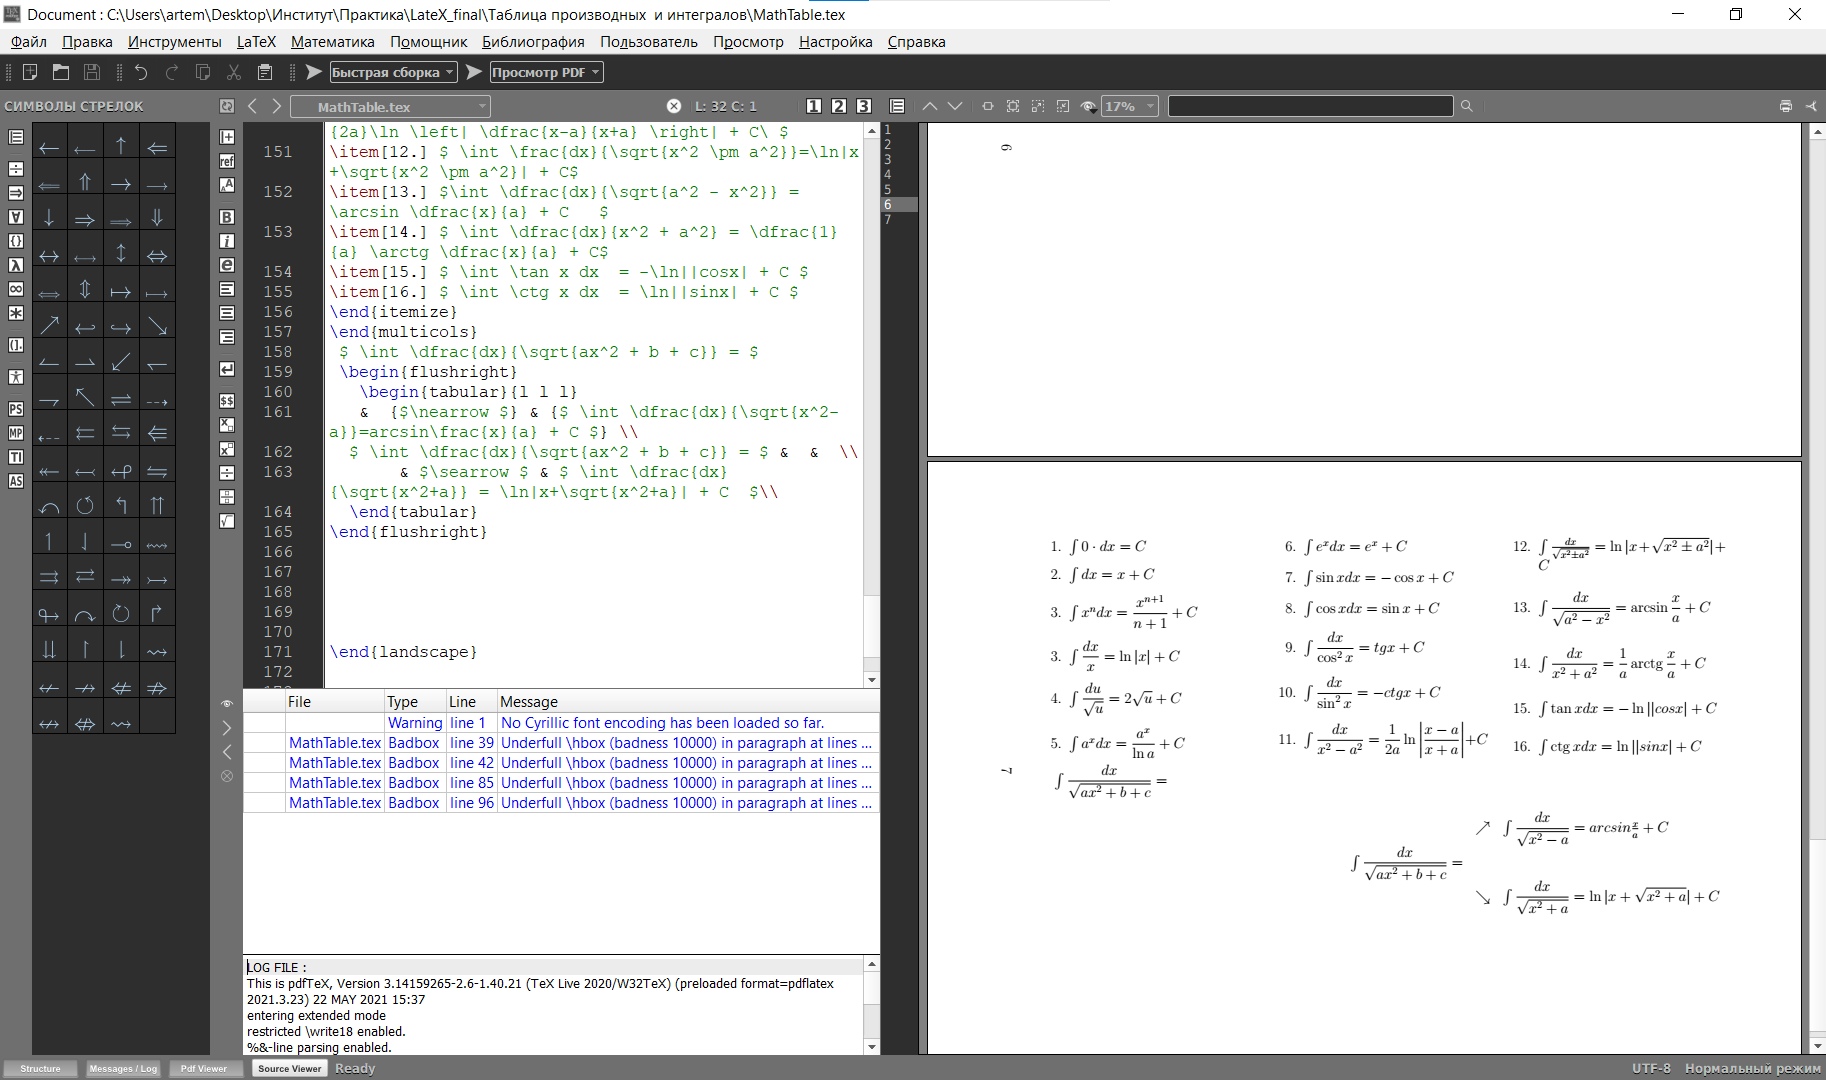
\includegraphics[width=15cm,height=9cm]{Example(1)}}%
\caption{Уже на этом этапе можно понять наскольно в \LaTeX \  проще и быстрее вводить математические формулы}
\label{fig:image}
\end{figure}
\newpage
Итак, быстро убедившись что ввод сложных математических формул не представляет трудностей мы приступили к вводу матриц и других крупных объектов.
\begin{figure}[h!]
\setlength{\fboxsep}{0pt}%
\setlength{\fboxrule}{1pt}%ширина рамки
\fbox{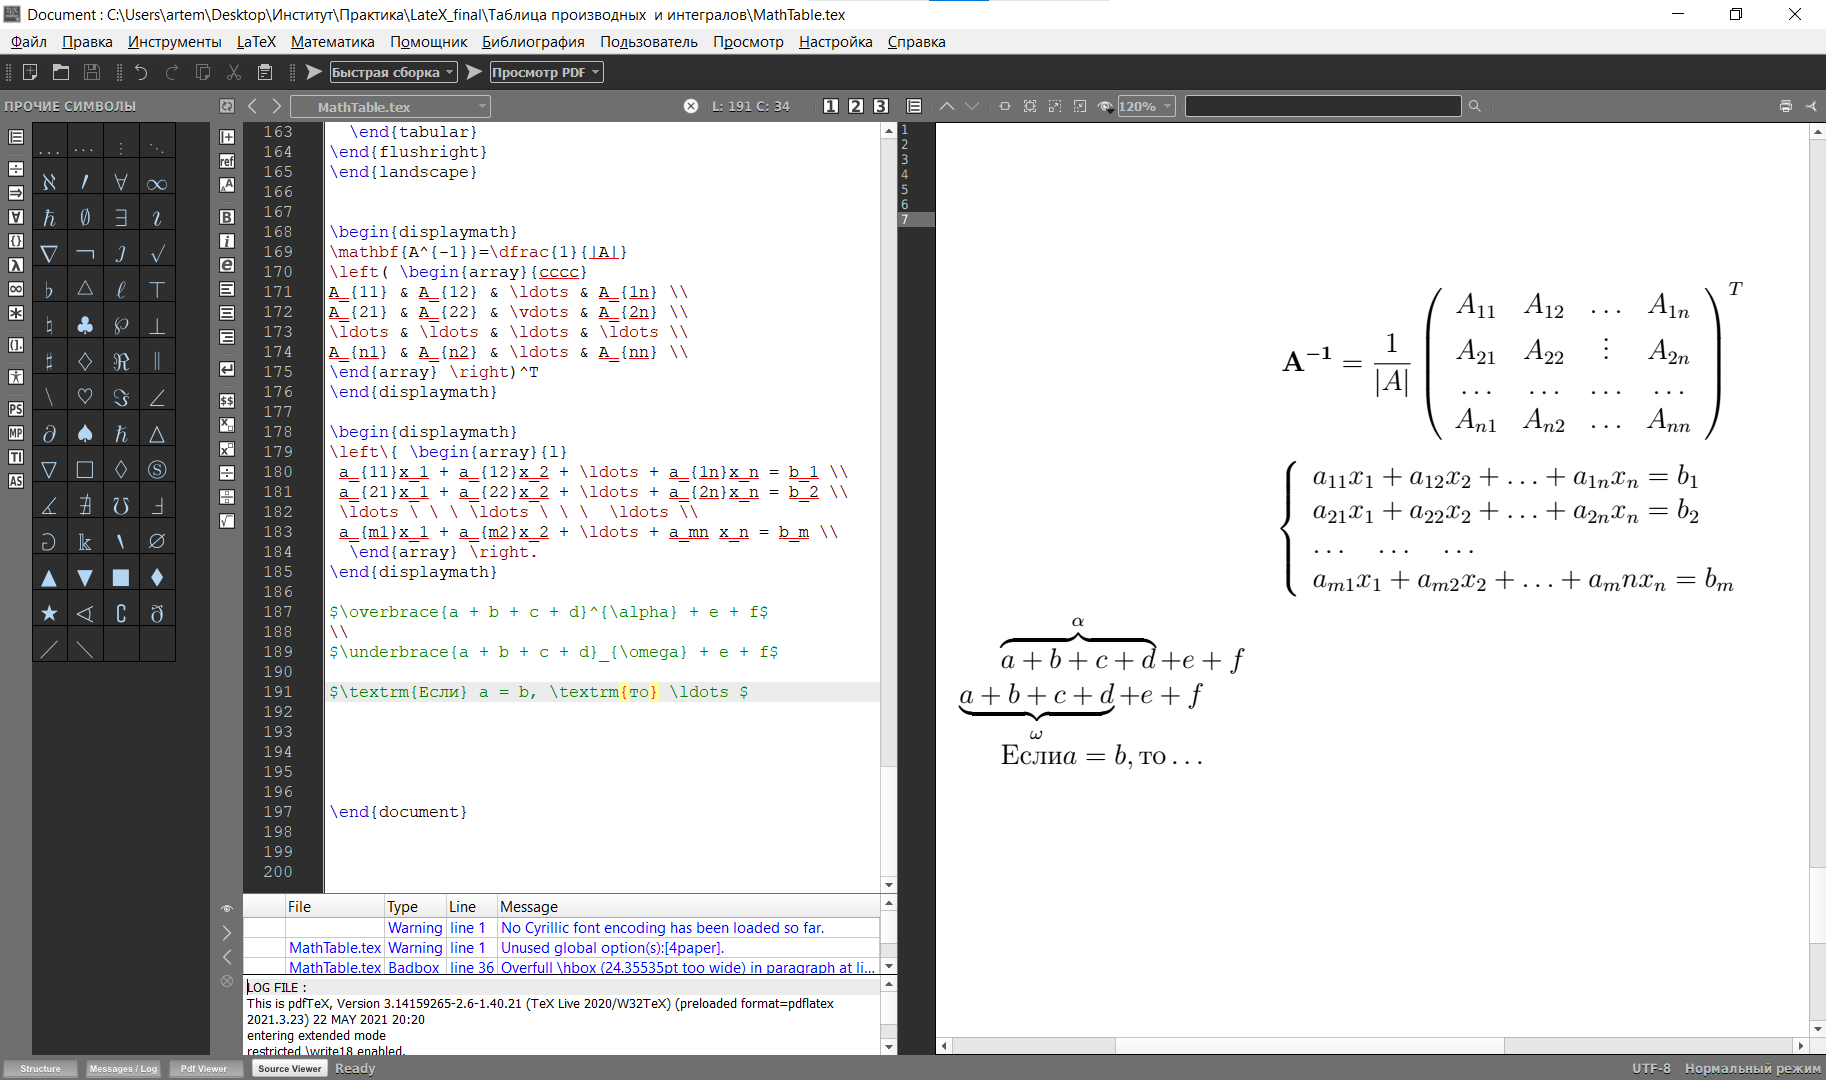
\includegraphics[width=15cm,height=9cm]{Matrrix(1)}}%
\caption{"Крупные' математические объекты}
\end{figure}
\\
Что же касается спец символов, в \LaTeX 'e их огромное количество,(к счастью) но раз уж речь идет о математике, то давайте попробуем собрать определение последовательности на языке " $\varepsilon \ \Delta $'
$$\lim_{x \rightarrow x_0}f(x) = A \  \Leftrightarrow \   \forall \ \varepsilon > 0, \ \exists \delta \ >0, |\forall x \ 0<|x-x_0|<\delta \ \Rightarrow |f(x) - A|< \varepsilon   $$


$$\lim_{x \rightarrow 0}\frac{\sin x}{x} = 1  $$

$$\lim_{x \rightarrow \infty} \left( 1 + \frac{1}{x} \right)^x = e  $$

%$\lim_{x \rightarrow 0} \dfrac{sinx}{x} = 1$

\subsection{16.04.21-28.04.21}
Для работы с графикой мы решили рассмотреть два пакета: \{graphicx\} и \{tikz\} первый служит для вставки растровых изображений в текст,  а второй позволяет выполнять построение различных геометрических фигур, блок-схем, а тыкже графиков некоторых функций, что представляет гораздо больший интерес. Начнем с пакета \{graphicx\}. \\
Для нам нужно подключить его в преамбуле документа:\\
\\
\hypertarget{D12}
$\backslash$\textbf{usepackage \{graphicx \}} \\
\textbf{\graphicspath\{\{pictures/ \}\} } Указываем название каталога где будут лежать изображения.(Он должен находиться в том же каталоге что и сам документ) Данная опция является необязательной, можно просто разместить все изображения в том же каталоге что и документ.\\
$\backslash$ \textbf{DeclareGraphicsExtensions\{.pdf,.png,.jpg\}} Указываем какие типы файлов будем использовать.Векторные изображения также поддерживаются. \\
Рассмотрим вставку изображений:\\
$\backslash$ \textbf{begin \{figure\}[h!]} "Обьявляем начало" изображения, в квадратных скобках указываем позицию изображения, "h!" обозначает, что изображение будет вставлено сразу после текста.       \\
$\backslash$ \textbf{ setlength \{ $\backslash$ fboxsep \} \{0pt \} } размер полей вокруг изображения     \\
$\backslash$ \textbf{setlength \{ $\backslash$ fboxrule \} \{ 1pt \} } ширина рамки \\
$\backslash$ \textbf{fbox \{ $\backslash$ includegraphics [ width=15cm,height=9cm ]\{ Matrrix \( 1 \) \} \} } задаем размеры изображения и указываем название файла(файл должен лежать в одной папке с документом)    \\%
$\backslash$ \textbf{caption \{ "Крупные' математические объекты \}}| Подпись под изображением  \\
$\backslash$ \textbf{end \{ figure \}  } "Конец" \\
Если подпись и рамка не трубуются, то достачно только строчки $\backslash$ \textbf{fbox \{ $\backslash$ includegraphics [ width=15cm,height=9cm ]\{ Matrrix \( 1 \) \} \} }. Вместо усазания размеров в сантиметрах можно использовать команду \textbf{scale} \( масштаб\). \\
Итак, перейдем к пакету \textbf{\{tikz\}}. Его базовая функция - начертание фигур по их координатам.\\
\begin{tabular}{lc}
$\backslash$ \textbf{begin\{tikzpicture\} }\\
$\backslash$\textbf{draw(0,0)--(1,0)--(1.5,-0.5)--(1.5,-2)--}\\
\textbf{(1,-3.5)--(2.5,-4.5)--(3,-4.5)}\\
\textbf{--(3,-4)--(2.5,-4)--(2,-3)}\\
\textbf{--(3,-2.5)--(3.5,-3.5)--(4.5,-4)}\\
\textbf{--(5,-4)--(5,-3.5)--(4.5,-3.5)}\\
\textbf{--(4,-3)--(4,-2.5)--(4.5,-3)}\\
\textbf{--(6.5,-3)--(7,-4.5)--(7.5,-5)--}\\
\textbf{(8,-5)--(8,-4.5)--(7.5,-4.5)}\\
\textbf{--(7.5,-3.5)--(8.5,-4.5)--(9,-4.5)}\\
\textbf{--(9,-4)--(8.5,-4)--(8,-3)--(8.5,-3)}\\
\textbf{--(9,-2.5)--(9,-1)--(8.5,-1.5)}\\
\textbf{--(8,-1.5)--(7.5,-1)--(7.5,-2)}\\
\textbf{--(7,-2)--(5,-1)--(4,-1)--(2.5,-1.5)}\\
\textbf{--(2.5,-0.5)--(1.5,0.5)--(1,0.5)--cycle;}\\
$\backslash$\textbf{ end \{ tikzpicture \}}\\
&
\begin{tikzpicture}
\draw(0,0)--(1,0)--(1.5,-0.5)--(1.5,-2)--(1,-3.5)--(2.5,-4.5)--(3,-4.5)--(3,-4)--(2.5,-4)--(2,-3)--(3,-2.5)--(3.5,-3.5)--(4.5,-4)--(5,-4)--(5,-3.5)--(4.5,-3.5)--(4,-3)--(4,-2.5)--(4.5,-3)--(6.5,-3)--(7,-4.5)--(7.5,-5)--(8,-5)--(8,-4.5)--(7.5,-4.5)--(7.5,-3.5)--(8.5,-4.5)--(9,-4.5)--(9,-4)--(8.5,-4)--(8,-3)--(8.5,-3)--(9,-2.5)--(9,-1)--(8.5,-1.5)--(8,-1.5)--(7.5,-1)--(7.5,-2)--(7,-2)--(5,-1)--(4,-1)--(2.5,-1.5)--(2.5,-0.5)--(1.5,0.5)--(1,0.5)--cycle;
\end{tikzpicture}
\end{tabular}
\\
\begin{tabular}{lr}

$\backslash$ \textbf{begin\{tikzpicture\}}\\
$\backslash$\textbf{draw(0,0)--(1,0.5)--(2.5,0.5)--(3,0)--(2,-0.5)}\\ \textbf{--(0.5,-0.5)--(0,0)--(0,-2.5)--(0.5,-3)--(0.5,-0.5)--(0.5,-3)--(2,-3})\\ \textbf{--(2,-0.5)--(2,-3)--(3,-2.5)--(3,0);}\\
$\backslash$ \textbf{draw[dashed](0,-2.5)--(1,-2)--(2.5,-2)--(3,-2.5);}\\
$\backslash$ \textbf{draw[dashed](1,-2)--(1,0.5);}\\
$\backslash$ \textbf{draw[dashed](2.5,-2)--(2.5,0.5);}\\
$\backslash$ \textbf{end \{ tikzpicture \}}\\
&
\begin{tikzpicture}
\draw(0,0)--(1,0.5)--(2.5,0.5)--(3,0)--(2,-0.5)--(0.5,-0.5)--(0,0)--(0,-2.5)--(0.5,-3)--(0.5,-0.5)--(0.5,-3)--(2,-3)--(2,-0.5)--(2,-3)--(3,-2.5)--(3,0);
\draw[dashed](0,-2.5)--(1,-2)--(2.5,-2)--(3,-2.5);
\draw[dashed](1,-2)--(1,0.5);
\draw[dashed](2.5,-2)--(2.5,0.5);
\end{tikzpicture}
\end{tabular}
\\
Все что нужно, это указывать координаты.При необходимости построить сложную фигуру можно строить несколько линий. Имеется возможность строить пунктирные линии, стрелки,также можно окрашивать в различные цвета,регулировать толщину.
\\
\begin{tabular}{lr}
$\backslash$ \textbf{begin\{tikzpicture\}[>=stealth]}\\            
$\backslash$ \textbf{draw[thick, ->,red](0,0)--(4,0);}\\
$\backslash$ \textbf{draw[thick, ->, red](0,0)--(1,3);}\\
$\backslash$ \textbf{draw[ultra thick, ->, blue](0,0)--(5,3);}\\
$\backslash$ \textbf{draw[dashed](4,0)--(5,3)--(1,3);}\\
$\backslash$ \textbf{end\{tikzpicture\}}\\
&
\begin{tikzpicture}[>=stealth]
\draw[thick, ->,red](0,0)--(4,0);
\draw[thick, ->, red](0,0)--(1,3);
\draw[ultra thick, ->, blue](0,0)--(5,3);
\draw[dashed](4,0)--(5,3)--(1,3);
\end{tikzpicture}
\end{tabular}

\vspace{3cm}
\textbf{Добавление подписей к прямым и углам}\\

\begin{tikzpicture}[scale=0.75]
\fill[left color=magenta, right color=yellow]
(0,0) -- node[below=3pt] {$a$} (4,0) --
node[right=5pt] {$b$} (4,3) --
cycle node[midway,above,sloped] {$c=\sqrt{a^2+b^2}$};
\node[below left] at (0,0) {\color{blue}$B$};
\node[below right] at (4,0) {\color{blue}$C$};
\node[above right] at (4,3) {\color{blue}$A$};
\end{tikzpicture}




\textbf{Окружности и дуги}\\

\begin{tabular}{lr}
$\backslash$ \textbf{begin\{tikzpicture\}} \\           
$\backslash$ \textbf{draw[Red,ultra thick](1,1) arc (20:60:2);}\\
$\backslash$ \textbf{draw[Red,ultra thick](0,0) arc (20:60:1.5);}\\
$\backslash$ \textbf{draw[thick](2,1) arc (0:-120:2);}\\
$\backslash$ \textbf{end\{tikzpicture\}}\\
&
\begin{tikzpicture}
\draw[Red,ultra thick](,1) arc (20:60:2);
\draw[Red,ultra thick](0,0) arc (20:60:1.5);
\draw[thick](2,1) arc (0:-120:2);
\end{tikzpicture}
\end{tabular}\\

В квадратных скобках указываются дополнительные параметры(как и для любых линий), затем указываются координаты центра, а затем название фигуры(в нашем случае это дуга) далее следуют градусные меры начала и конца, длина радиуса.\\
\begin{tabular}{lr}
$\backslash$ \textbf{begin\{tikzpicture\}} \\           
$\backslash$ \textbf{ draw[fill=Red] (0,0) circle (1); }\\
$\backslash$ \textbf{ [color=green, outer color=Blue] (2,0) circle (1);}\\
$\backslash$ \textbf{[ball color=green](1,-1.7) circle (1);}\\
$\backslash$ \textbf{end \{tikzpicture\}}\\
&
\begin{tikzpicture}
\draw [fill=Red] (0,0) circle (1);
\draw [color=green, outer color=Blue] (2,0) circle (1);
\draw [ball color=green] (1,-1.7) circle (1);
\end{tikzpicture}
\end{tabular}


В пакете \textbf{\{tikz\}} имеется огромное количество готовых фигур, однако перечислять их мы не будем, ибо на это ушло бы слишком много времени. Однако мы не можем не показать использование данного пакета для построения графиков функций.(как предустановленных, так и при помощи таблицы значений)


\begin{tikzpicture}
		\begin{axis}[
			title = Кубическая парабола,
			xlabel = {$x$},
			ylabel = {$y$},
			grid = both,
			minor tick num = 2
			]
			\addplot[magenta] {x^3};
		\end{axis}
	\end{tikzpicture}
\vspace{2cm}
\begin{tikzpicture}
\begin{axis}
grid = both,
\addplot3 table [x = b, y = a, z = c] {
	a      b      c
	1      1      1
	7      3      4 
	3      9      5 
	4      8      6
	5      2      7
};
\end{axis}
\end{tikzpicture}
\vspace{2cm}
\begin{tikzpicture}
    \begin{axis}[
    axis x line = center,
    axis y line = center,
    minor x tick num=1,
    xlabel={$x$},
    xmin=-10,xmax=10,
    ylabel={$y$},
    ymin=-10,ymax=10,  
    ]
    \addplot[magenta] {x^3};
    \end{axis}
\end{tikzpicture}
\vspace{2cm}
\begin{tikzpicture}
\begin{axis} [
    legend pos = north west, 
    ymin = 0, 
    grid = major
]
\legend{ 
	$\log_2(x)$, 
	$\ln(x)$, 
	$\log_{10}(x)$
};
\addplot {log2(x)};
\addplot {ln(x)};
\addplot {log10(x)};
\end{axis}
\end{tikzpicture}
\vspace{2cm}

\begin{tikzpicture}
\begin{axis}
\addplot3[
    surf,
] 
coordinates {
(0,0,0) (0,1,0) (0,2,0)

(1,0,0) (1,1,0.6) (1,2,0.7)

(2,0,0) (2,1,0.7) (2,2,1.8)
};
\end{axis}
\end{tikzpicture}

Как можно заметить, из последнего примера пакет textbf{tikz} позволяет выполнять построение 3D объектов. Однако, мы не стали затрагивать его слишком подробно, ибо не обладаем столь глубокими познаниями в геометрии. 

\subsection{29.04.21-14.05.21}
Приступили к составлению финального отчета. Выравние текста выполняется при помощи окружений 
\textit{\textbf{``left' ``center' ``right'}}. Окружения это особый вид команд, позволяющий использовать специальные правила оформления больших частей текста или выполнять построение различных объектов. Окружения влияют на текст заключенный между командами начала и конца(\textit{\textbf{``$\backslash$begin\{имя окружения\}' ``$\backslash$end\{имя окружения\}' }} окружения и могут быть вложенными. Очень полезным для нас оказались окружения \textit{\textbf{``tabular'}} \ и \textit{\textbf{``table'}}(отличаются тем что в \textit{\textbf{``table'}} отсутствует разметка и \textit{\textbf{``tabular'}} может быть ``вложен' в \textit{\textbf{``table'}} ) которое должно служить для составления таблиц. Однако пригождаются и для других целей:

\begin{figure}[h!]
\setlength{\fboxsep}{0pt}%
\setlength{\fboxrule}{2pt}%ширина рамки
\fbox{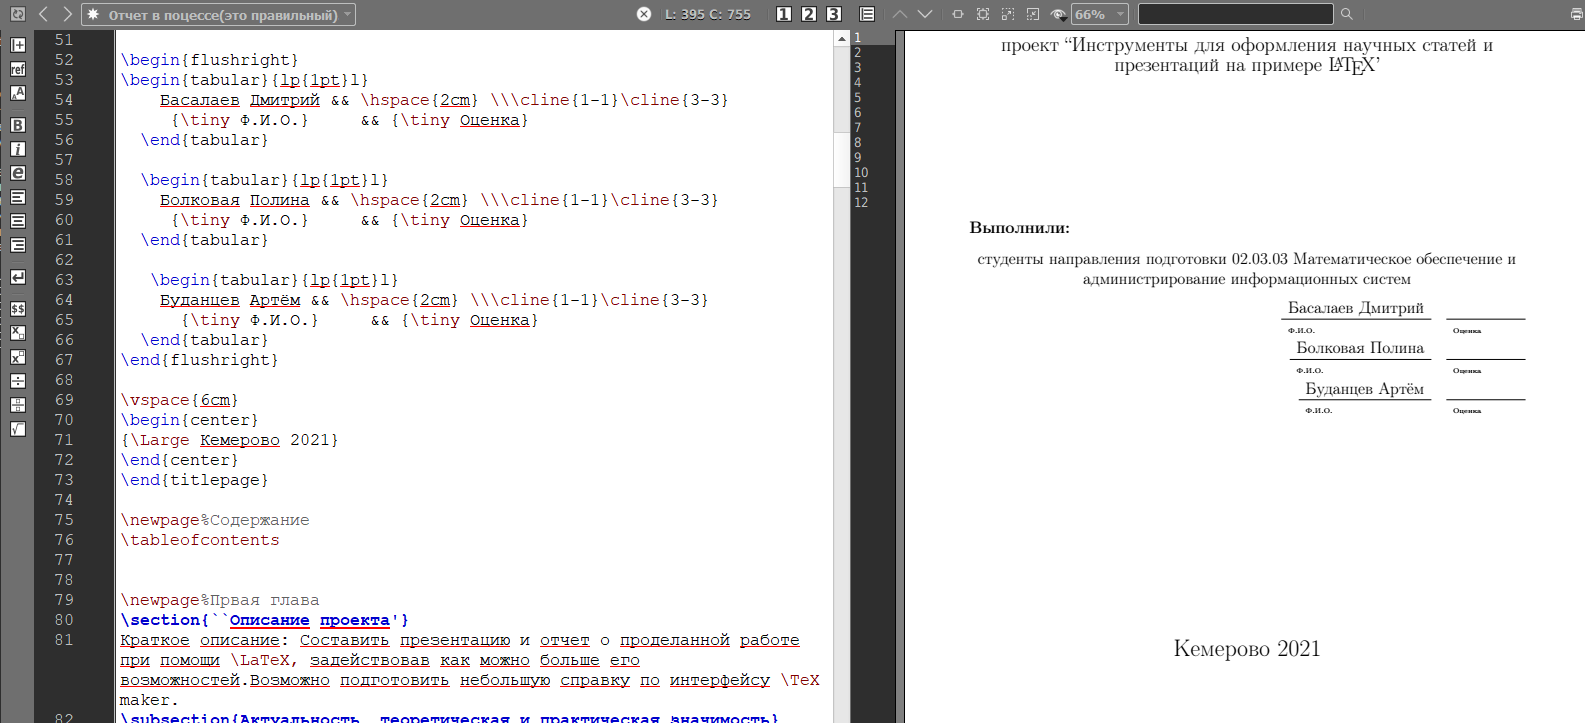
\includegraphics[scale=0.5]{Let's_talk_about_Table}}%
\caption{Например на титульном листе}
\end{figure}

\newpage

\begin{figure}[h!]
\setlength{\fboxsep}{0pt}%
\setlength{\fboxrule}{2pt}%ширина рамки
\fbox{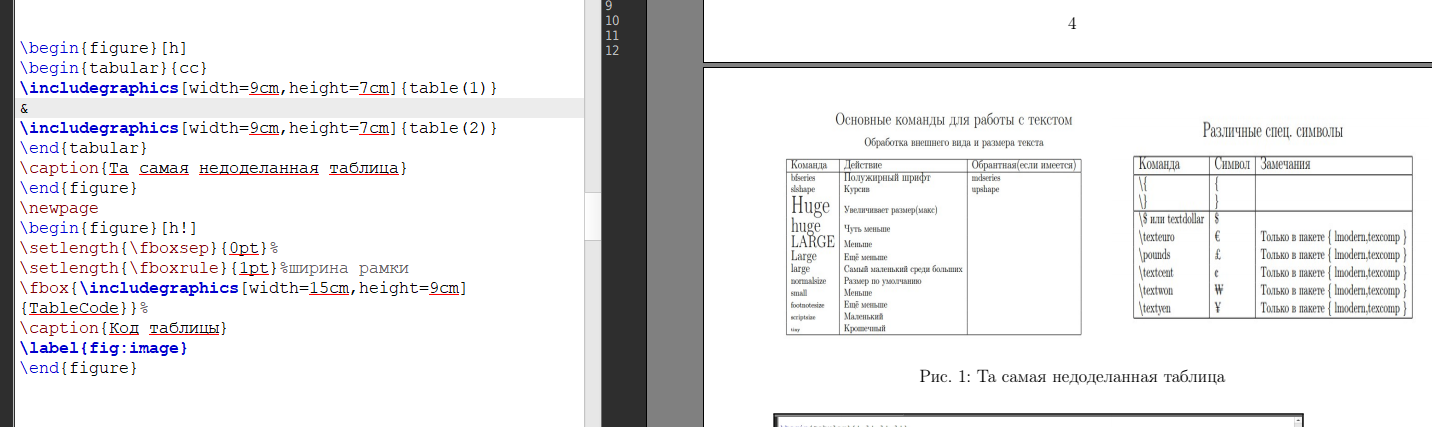
\includegraphics[scale=0.5]{Let's_talk_about_tables(2)}}%
\caption{Также полезно при вставке изображений}
\end{figure}

\begin{figure}[h!]
\setlength{\fboxsep}{0pt}%
\setlength{\fboxrule}{2pt}%ширина рамки
\fbox{\includegraphics[scale=0.5]{Let's_talk_about_tables(3)}}%
\caption{С его помощью даже можно рисовать таблицы}
\end{figure}

Ещё одно ``Простое окружение' \textsl{\textbf{itemize}} \ служит для составления списков.(+ по сравнению с Word: можно вручную вписывать маркеры)
\begin{verbatim}
\begin{itemize}
  \item[а сюда можно вписывать маркеры
  (по умолчанию это точки)]
   Level 0 Item 0 
  \item Level 0 Item 1 
  \begin{itemize}
    \item Level 1 Item
    \begin{itemize}
      \item Level 2 Item
      \begin{itemize}
        \item Level 3 Item
      \end{itemize}
    \end{itemize}
  \end{itemize}
\end{itemize}

Также есть нумерованный список:

\begin{enumerate} 
  \item первый элемент первого уровня содержит список 
    \begin{enumerate} 
        \item элемент списка второго уровня
        \item второй элемент списка второго уровня
    \end{enumerate} 
  \item  второй элемент первого уровня
\end{enumerate} 
\end{verbatim}



Также мы ознакомились с окружением \textit{\textbf{``scope'}} \ которое является вспомогательным к \textit{\textbf{``tikzpicture'}} \ и служит для работы с tikz рисунком как с единым объектом.(масштабирование, позиционирование)

\begin{figure}[h!]
\setlength{\fboxsep}{0pt}%
\setlength{\fboxrule}{2pt}%ширина рамки
\fbox{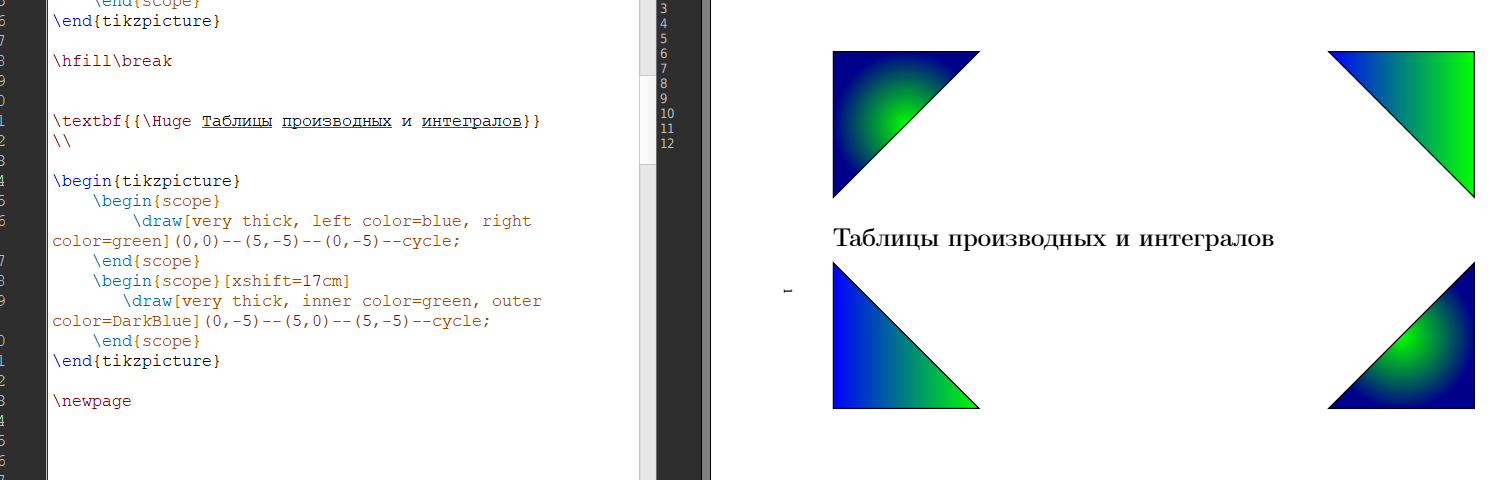
\includegraphics[scale=0.5]{Scope}}%
\caption{Однако в основном отчете оно нам не пригодилось}
\end{figure}

\begin{minipage}[c][2cm][c]{9cm} 
Эта строка внутри ``minipage'
\end{minipage}
В полном соответствии со своим названием окружение \textsl{\textbf{minipage}} создает страницу внутри страницы, которая может содержать свои собственные сноски, абзацы, а также окружения \textsl{\textbf{ array, tabular и multicols.}} Кроме того,\textsl{\textbf{minipage}} можно использовать внутри плавающих объектов, создаваемых окружениями \textsl{\textbf{figure}} и \textsl{\textbf{table}}, добиваясь весьма интересных эффектов.

Параметр \underline{pos} может принимать одно из трех значений — \underline{c, t или b} и управляет вертикальным выравниванием блока по отношению к базовой линии окружающего текста — по центру, по верхнему и по нижнему краю соответственно. \underline{height} определяет высоту, а \underline{width} — ширину блока. Параметр contentpos управляет расположением содержимого по вертикали внутри блока, и принимает уже знакомые значения \underline{c, t и b}.

Также крайне полезным оказалось окружение \textsl{textbf{verbatim}} \ в зоне его действия текст не воспринимается как команды, все пробелы и отступы отображаются ``как есть' а также не учитывается разметка страницы. При помощи этого окружения очень легко вставить в документ код практически на любом языке программирования.(имеются даже опции для подсветки синтаксиса)





\footnote{Кстати тут есть сноски, не знаю стоит ли это упоминать(ибо мы ими опять таки не пользовались)}

Также в \LaTeX можно реализовать одно из важных примуществ pdf документов - ссылки. Если подключить пакет \textsl{\textbf{hyperref}} то автособираемое автоматически превратится в набор ссылок(что очень удобно) Также можно рассавлять ссылки вручную: % якорь для ссылок на это определение
\newpage
\hyperlink{D12}{смотреть здесь!}
\begin{verbatim}
\hypertarget{d6(а это уникальный номер ссылки)} 
{Это якорь, сюда будет указывать ссылка}

\hyperlink{d6(это уникальный номер ссылки)}{А это текст самой ссылки}
\end{verbatim}

\subsection{15.05.21-}
Приступили к составлению этого отчета и презентации.



\section{Выводы}


\section{Литература}
\begin{enumerate} 
\item Львовский С. М. Набор и вёрстка в системе \LaTeX. — М.: МЦНМО, 2006. — 448 с.
\item Котельников И. А., Чеботаев П. З. \LaTeX по-русски. — СПб. : «Корона-Век», 2011. — 496 с.
\item А.А. Жидков Интерактивные презентации в системе \LaTeX
Учебно-методическое пособие
\item Курс «Документы и презентации в LaTeX (Introduction to \LaTeX)» на сайте \url{coursera.org - https://www.coursera.org/learn/latex/home/welcome}
\end{enumerate}

\end{document}
